\clearpage
\newpage 
\section{Supplementary Materials for Experiments}\label{appendix:fine_grained_resumgrpo}

In this section, we supplement the fine-grained experimental analysis of ReSum-GRPO, including training efficiency, inference costs, and concrete cases. 


\subsection{Training Efficiency}
\begin{table}[!h]
    \centering
     \caption{\textbf{Comparison of average time per single gradient update step across RL algorithms.} Each step is configured with \texttt{batch\_size}$=64$ and $G=8$, optimizing over 512 collected trajectories.}
   \resizebox{0.6\linewidth}{!}{

    \begin{tabular}{c|c|c|c}
      \toprule
      \rowcolor{COLOR_MEAN} \textbf{Model} & \textbf{Device} & \textbf{GRPO} & \textbf{ReSum-GRPO} \\  \midrule
       WebSailor-3B  & 8×144GB GPUs & 0.62 Hours & 1.05 Hours \\
       WebSailor-7B & 8×144GB GPUs & 0.96 Hours & 1.44 Hours \\ 
       WebSailor-30B & 16×144GB GPUs & 0.94 Hours & 1.25 Hours \\ \bottomrule
    \end{tabular}
   }
    \label{tab:rl_training_time}
\end{table}

We provide the required devices and the average time for each training step for both RL algorithms in Table~\ref{tab:rl_training_time}. Compared with GRPO, ReSum-GRPO modifies long trajectories by segmenting them based on summarization and then resumes the conversation for continued exploration. Consequently, the times required for both trajectory collection and policy model updates are lengthened. Based on the statistics in the table, ReSum-GRPO roughly increases training time by approximately 33\% to 69\% compared with GRPO, which is acceptable.


\subsection{Inference Costs}

\begin{figure}[!h]
    \centering
    \begin{subfigure}[b]{0.35\textwidth}
        \centering
        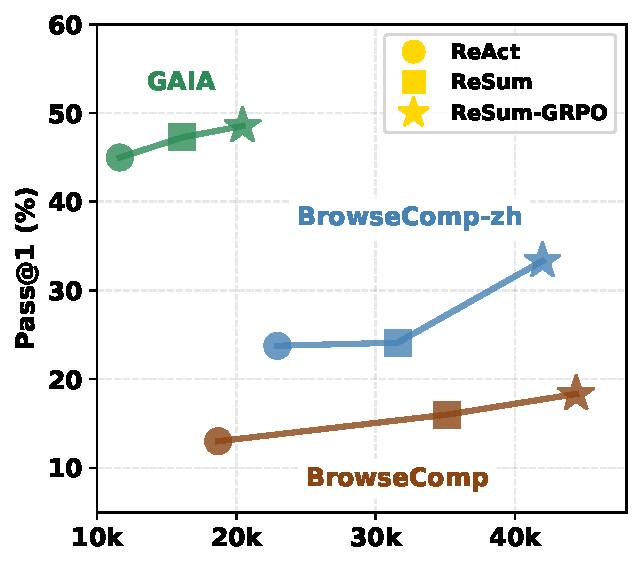
\includegraphics[width=\textwidth]{images/websailor30b_tool_token.pdf}
         \caption{Number of cost tokens vs. Performance}
         \label{fig:token_comp_3mode}
    \end{subfigure}
    \begin{subfigure}[b]{0.35\textwidth}
        \centering
        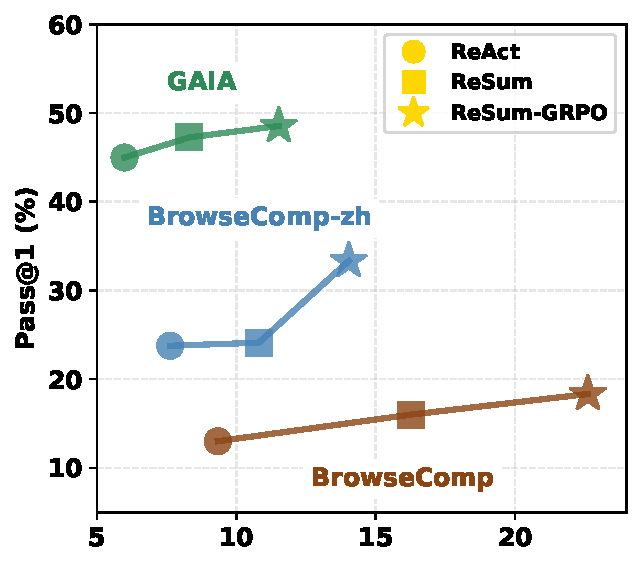
\includegraphics[width=\textwidth]{images/websailor30b_tool_call.pdf}
        \caption{Number of tool calls vs. Performance}
        \label{fig:toolcall_3mode}
    \end{subfigure}
     \caption{\textbf{Resource consumption vs. performance across different paradigms.} We compare three paradigms: training-free ReAct, training-free ReSum, and ReSum-GRPO, consistently using WebSailor-30B. ReSum paradigms achieve higher performance with acceptable resource utilization across all benchmarks.}
\end{figure}

We further analyze resource consumption, i.e., the average number of tokens and tool calls required to correctly solve a query across different inference paradigms: training-free ReAct, training-free ReSum, and ReSum after ReSum-GRPO training. Token consumption refers to the total number of tokens in a complete trajectory for a query. Here, we only consider trajectories that successfully lead to a correct final answer. The results for WebSailor-30B across various benchmarks are presented in Figures~\ref{fig:token_comp_3mode} and~\ref{fig:toolcall_3mode}. From these results, we observe that in the training-free setting, ReSum significantly boosts performance with only marginal increases in resource costs compared to ReAct. Following targeted ReSum-GRPO training, agents become more inclined to rely on summaries for continued reasoning, which, while incurring additional resource costs, leads to even higher performance. Notably, ReSum paradigms achieve substantial performance improvements while maintaining resource costs within a reasonable range, e.g., typically $\sim$2x the original costs.


\subsection{Efficiency Comparison with MEM1}\label{appendix:mem1_cost} 

\begin{figure}[!h]
    \centering
    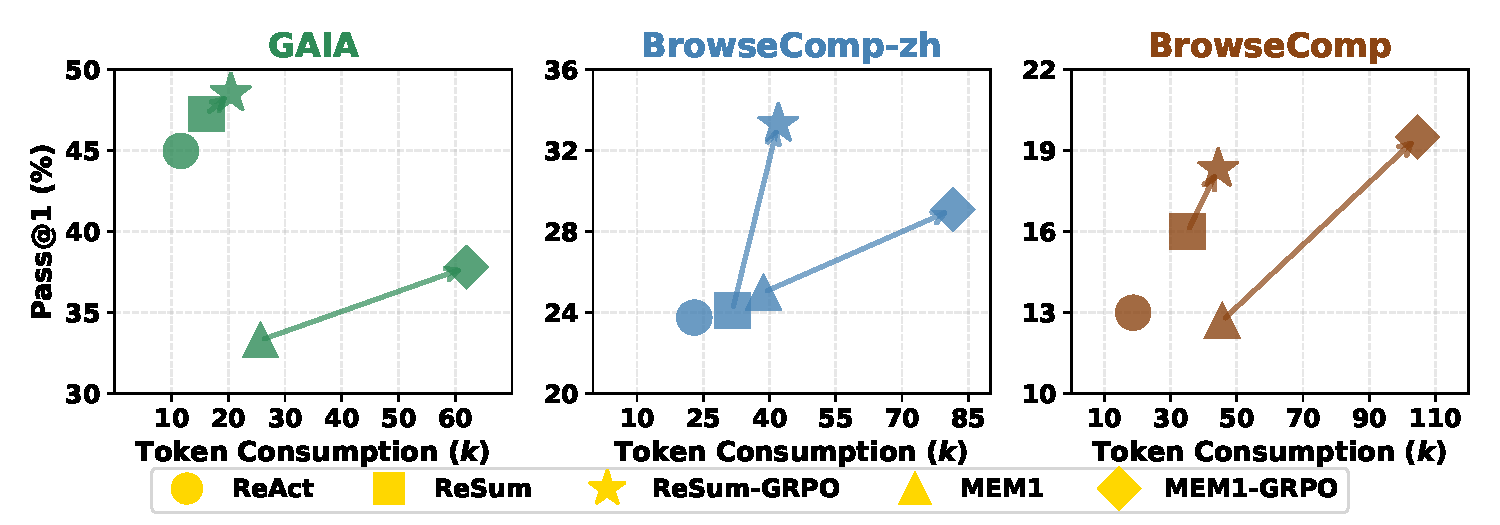
\includegraphics[width=0.75\linewidth]{images/resum_mem1_comparison.pdf}
    \vspace*{-8pt}
    \caption{\textbf{Trade-off between average token consumption and performance across ReSum and MEM1 paradigms.} Token consumption is calculated as the average total number of tokens required for a successful trajectory.}
    \label{fig:mem1_cost}
\end{figure}

In this subsection, we evaluate the inference efficiency of the ReSum and MEM1 paradigms by comparing their total token consumption against performance under both training-free and RL-trained settings. As illustrated in Figure~\ref{fig:mem1_cost}, MEM1 incurs substantial token overhead, particularly after targeted MEM1-GRPO training. This surge in cost is attributed to its iterative architecture, which requires continuous cycles of reasoning, memory consolidation, and tool invocation. In contrast, ReSum demonstrates a superior efficiency-performance balance. Notably, ReSum-GRPO achieves comparable or even higher success rates while consuming fewer tokens than MEM1-GRPO, highlighting its practicality for resource-constrained deployment.
